\chapter{Analisi e altri possibili approcci fingerprint based}

Nei capitoli precedenti è stato osservato  come l'utilizzo di un agente  e delle relative funzionalità di HIDS possano essere utilizzate per  aumentare il panorama di caratteristiche analizzabili di un sistema e incrementarne di conseguenza la sicurezza.

Dalle analisi condotte sulle due botnet, emerge che sono stati utilizzati principalmente software IDS che utilizzino strumenti di rilevazione basati su tecniche di pattern matching, prediligendo quindi l'approccio fingerprint based.
Come osservato nel \Cref{IDS}, gli approcci fingerprint based funzionano molto bene per malware e attività malevole per cui esista già una firma identificativa al momento della rilevazione. Nello studio  effettuato su UBoat (\Cref{uboat}) si può osservare come le regole create per l'identificazione della botnet siano basate su caratteristiche peculiari del software analizzato. Piccole variazioni o l'offuscamento all'interno del codice del  payload, potrebbero rendere parte delle regole di rilevazione create inefficienti verso la nuova versione del software malevolo. Ad esempio, se il botmaster distribuisse una nuova versione del payload, che durante la fase operativa di instaurazione della persistenza inserisce una copia dell'eseguibile nel sistema con un nome o una posizione differenti da quelle specificate, si potrebbero perdere gli allarmi relativi a tale evento.
Complicazioni aggiuntive come la cifratura del traffico di rete e tecniche di \textit{detection evasion} possono rendere ancora più ardua la rilevazione.

Va considerato anche che le attività degli host monitorati potrebbero generare molta attività di log rendendo le rilevazioni molto rumorose e spesso difficili da analizzare.
Inoltre come già precedentemente osservato, tale approccio non può essere applicato in caso di malware zero-day. Per cercare di ovviare a queste problematiche i ricercatori e vendor di sistemi di sicurezza informatici, cercano di tenere i database di fingerprint  il più aggiornati possibile oltre a ricercare nuove tecniche principalmente basati su rilevazioni di anomalie.

Tra le tecniche e le possibilità di rilevazione  fingerprint based analizzate, che sarebbe possibile integrare facilmente all'interno dell'infrastruttura di testing sviluppata, vi sono:
\begin{itemize}
    \item Yara rules;
    \item Integrazione con virus engine;
    \item API calls.
\end{itemize}

\smallskip
Yara \cite{yara} è un tool utilizzato per ricercare e classificare malware. Attraverso Yara è possibile creare descrizioni, anche dette regole, basate su pattern testuali o binari.
Le YARA rule sono scritte in una sintassi specifica che permette di definire una serie di criteri di ricerca per individuare un determinato oggetto o comportamento. Ogni regola YARA è composta da tre sezioni principali:
\begin{description}
    \item [Meta] Contiene il nome della regola e altre informazioni, come l'autore, la data di creazione e la descrizione della regola stessa.
    \item [Strings] Contiene i pattern che vengono utilizzati all'interno della sezione Condition.
    \item [Condition] La parte centrale della regola che definisce il criterio di ricerca da applicare. La condizione è composta di un'espressione booleana e di stringhe su cui eseguire il match.
\end{description}

Un esempio di Yara rule è il seguente \cite{yaraexample}:
\begin{lstlisting}[caption={Esempio di Yara rule.},captionpos=b,frame=single]
rule silent_banker : banker
{
    meta:
        description = "This is just an example"
        threat_level = 3
        in_the_wild = true

    strings:
        $a = {6A 40 68 00 30 00 00 6A 14 8D 91}
        $b = {8D 4D B0 2B C1 83 C0 27 99 6A 4E 59 F7 F9}
        $c = "UVODFRYSIHLNWPEJXQZAKCBGMT"

    condition:
        $a or $b or $c
}
\end{lstlisting}


All'analisi di un file, la regola in esempio, andrà alla ricerca dei pattern binari e testuali elencati nella sezione Strings e nel caso almeno uno venisse trovato la regola darebbe esito positivo e il file sarebbe etichettato come \textit{silent\_banker}.
\smallskip
Le Yara rule sono utilizzate all'interno di Strelka in Security Onion per la ricerca di file malevoli all'interno del traffico di rete. Questo approccio può essere importato all'interno dell'host da monitorare. Attraverso Wazuh, per esempio, è possibile integrare Yara con il modulo di File Integrity Monitoring dell'agent. Così facendo, ogni volta che viene modificato un file monitorato Yara effettuerà una scansione su di esso alla ricerca di file malevoli sfruttando le Yara rule.

\medskip
%integrazione con altri virus engine
%api call stuff
%leggere paper per altri approcci ids per vedere se c'è qualcosa di interessante
%behavior baased IDS

%In questo modo il server può ricevere informazioni ed eventi da un infinita lista di possibili sorgenti.

Per aumentare ulteriormente la sicurezza degli end-point è possibile integrare sistemi antivirus o simili, sfruttando le capacità di inoltro dei log degli agent o di altri software.  Wazuh ad esempio, all'interno della propria documentazione cita ClamAV \cite{clamav} come possibile alternativa open source di software antivirus multi piattaforma, basato su fingerprint. Esso è in grado di supportare diversi tipi di signature per analizzare molteplici formati di file, compresi archivi ed email.

Su un sistema Windows può essere utile sfruttare i log di Windows Defender\footnote{antivirus installato di default all'interno dei sistemi operativi Windows.} per avere visibilità delle infezioni rilevate da esso o per analizzare i risultati di possibili scansioni effettuate.

Un'ultima menzione è la possibilità di integrazione del modulo di File Integrity Monitoring degli agent Wazuh con il servizio VirusTotal \cite{virustotal}. VirusTotal è un sistema che sfrutta più di 70 antivirus/scanner e molteplici liste di domini/IP malevoli, per eseguire l'analisi di file online direttamente dal portale web del servizio. Esso offre inoltre un API utilizzabile per sfruttare il servizio programmaticamente. Grazie all'integrazione con Wazuh, quando l'agente segnala un cambiamento, una creazione o una cancellazione di un file, il server  utilizza l'API di VirusTotal per inoltrare l'hash del file e ricevere i risultati dell'analisi da esso effettuata.

In conclusione, questi sono solo alcuni dei rilevanti esempi di integrazione che è possibile effettuare per aumentare ulteriormente l'analisi su un sistema. Il vasto mercato dei sistemi di sicurezza lascia un'ampia scelta all'amministrazione della sicurezza, permettendo di personalizzare ulteriormente il livello di protezione del sistema.


\medskip

%api hooking poi conclusione
 
\label{apihooking}
Per quanto riguarda le API call invece, si è voluto testare  uno dei meccanismi utilizzato da molti  Endpoint Detection and Response (EDR) e antivirus, per il monitoraggio di  processi in real-time alla ricerca di comportamenti malevoli.  
La tecnica in questione è chiamata API hooking. 

L'API hooking  consente di monitorare e intercettare le chiamate ad una o più API call di un sistema operativo o di un'applicazione, per modificare o estendere il loro comportamento. In pratica, l'API hooking consente di intercettare la comunicazione tra un'applicazione e il sistema operativo, permettendo di monitorare e modificare il comportamento dell'applicazione o del sistema operativo stesso, ad esempio per rilevare e prevenire attacchi informatici. Gli sistemi di sicurezza sfruttano questa tecnica per intercettare API call comunemente utilizzate da malware per osservarne il comportamento alla ricerca di pattern sospetti.

L'idea di fondo era sfruttare questa tecnica per monitorare le chiamate di sistema di un software alla ricerca di pattern nell'ordine o insieme di chiamate effettuate. 


%spiegare api hooking
Entrando nei dettagli, un possibile  esempio di hooking di chiamata di  funzione in un processo a 32 bit può essere il seguente \cite{hooking1,hooking2}:
\begin{enumerate}
    \item Si estrae l'indirizzo in memoria della funzione di cui si vuole eseguire l'hook;
    \item Vengono salvati i primi 5 byte  della funzione;
    \item Si crea la funzione a cui passerà il controllo quando la funzione di cui si vuole eseguire l'hook viene chiamata, che chiameremo \textit{HookedFunction}. Prima che questa finisca la propria esecuzione, riscriverà i byte  precedentemente salvati al loro posto, per poi eseguire la funzione originale;
    \item Si estrae l'indirizzo in memoria della HookedFunction;
    \item Si sovrascrivono i primi 5 byte della funzione originale con gli opcode di jump assoluto o relativo all'indirizzo della HookedFunction.
\end{enumerate}

Questo è il modo più banale di eseguire tale operazione, in quanto ad ogni esecuzione della funzione di cui si esegue l'hook i 5 byte di partenza vengono sovrascritti più volte. Un implementazione più efficiente può essere ottenuta sfruttando i cosiddetti \textit{trampolini}. Un trampolino è una funzione che esegue quanto segue \cite{hooking2}:
\begin{enumerate}
    \item Esegue i byte originali precedentemente salvati della funzione di cui è eseguito l'hook;
    \item Salta all'interno del codice della funzione originaria, dopo l'istruzione di jump inserita manualmente.
\end{enumerate}

Tuttavia tale operazione richiede la gestione del caso in cui la sovrascrittura dei 5 byte iniziali dovessero rompere la sintassi della restante porzione di codice.

Comunque in entrambi i casi, quando la funzione da monitorare viene eseguita, il controllo passerà alla funzione da noi definita per poi tornare ad eseguire la funzione originale.

Le cose sono però più complicate in processi a 64 bit, dato che le funzioni potrebbero essere posizionate tra loro troppo distanti per far sì che siano raggiungibili con un jump relativo a 32 bit. Dato che non esistono jump relativi a 64 bit, si potrebbe pensare di usare un jump assoluto ad un indirizzo di memoria preciso a 64 bit.  Tuttavia tale salto richiede almeno 13 byte di opcode, e quindi tale approccio non sarebbe utilizzabile per funzioni che abbiano meno di 13 byte da sovrascrivere.

Per risolvere questo problema si può eseguire un salto relativo a 32 bit, che richiede 5 byte di opcode, ad una porzione di codice allocata in  vicinanza (così che sia raggiungibile con un salto relativo) e quindi eseguire il jump assoluto all'indirizzo della HookedFunction.

\smallskip


Wazuh offre la possibilità di monitoraggio di API call su Linux sfruttando l'integrazione con l'Audit System del sistema operativo. Tuttavia, dato che la botnet su cui si sarebbe voluto effettuare il test (UBoat) può eseguire solo su Windows è stato ricercato un software alternativo che servisse allo scopo.

Inizialmente è stato utilizzato WinAPIOverride \cite{winapioverride}, un tool di monitoraggio e hooking di API call per processi a 32 e 64 bit.
Questo offre anche un tool per l'estrazione di tutte le API call effettuate da un software, così che risulti più facile estrarne una possibile fingerprint per i nostri scopi.
A basso livello esso utilizza un Kernel driver rendendo quindi possibile intercettare ogni chiamata di sistema senza dover iniettare codice in applicativo.
Specificando quali API call si desiderasse monitorare e caricando un DLL contenenti le strutture dati con le funzioni sui cui eseguire l'hook e le funzioni a cui ridirigerle, WinAPIOverride si preoccupava di eseguire l'hooking.
All'interno della sezione di codice \ref{winapioverride} è possibile vedere un esempio di struttura dati utilizzata in cui viene specificata l'API call sul quale eseguire l'hook, in questo caso Sleep della libreria kernel32.dll, e la funzione a cui reindirizzare il flusso di esecuzione con relativi parametri.
\lstset{xleftmargin=0cm}
\begin{lstlisting}[frame=single,caption={esempio di struttura dati per hook in WinAPIOverride.},captionpos=b,label={winapioverride}]
STRUCT_FAKE_API_WITH_USERPARAM pArrayAfterAPICall[] =
{    
	{_T("kernel32.dll"),_T("Sleep"),(FARPROC)MyFunction,
            StackSizeOf(DWORD) ,0,0},
	{_T(""),_T(""),NULL,0,0,0}
};
...
\end{lstlisting}

Seppure il programma funzionasse correttamente, la licenza gratuita del tool non permette l'utilizzo su macchina virtuale. Per questo motivo è stato deciso di implementare un piccolo prototipo d'esempio senza l'ausilio di strumenti di terze parti, che sarebbe quindi potuto essere testato su macchina virtuale. Il prototipo è stato tenuto il più semplice possibile in quanto il fine ultimo era il consolidamento di quanto appreso riguardo la tecnica di hooking.
Lo scopo del prototipo è intercettare le API call di un  processo in esecuzione e di inviare un log al Windows Event Log System per notificarne l'accaduto, così che l'agente Wazuh potesse inviare tale log al Server per ulteriore analisi e intrusion detection.

\medskip
%spiegare DLL injetction
%foto prototipo 
Senza il supporto del tool era necessario trovare un modo per poter eseguire il codice, necessario per svolgere le attività di hooking, all'interno del processo da monitorare. Per evitare di dover scrivere un Kernel driver da zero in modo simile a  WinAPIOverride, è stato deciso di utilizzare una tecnica chiamata DLL injection, cui fine è l'esecuzione di codice arbitrario all'interno di un processo. Vi sono molti modi per effettuare ciò.
La versione di tecnica utilizzata consiste nel forzare un processo ad eseguire un thread, che è incaricato di caricare  all'interno del contesto del processo una DLL \cite{dllinjection}. Il caricamento di una DLL comporta come detto, tra le cose, l'esecuzione nel contesto del processo del codice contenuto all'interno del \textit{DllMain} della libreria. 

Ricapitolando quindi, inserendo  il codice responsabile dell'hooking all'interno della DLL è possibile eseguirlo attraverso DLL injection all'interno del processo così monitorato.

Entrando nei dettagli, l'implementazione si compone dei seguenti punti:
\begin{enumerate}
    \item Si ottiene l'handle del processo che si desidera monitorare;
    \item Si alloca memoria all'interno del processo;
    \item Si scrive all'interno della memoria riservata  il path al DLL da iniettare;
    \item Si ottiene l'indirizzo in memoria della funzione di libreria utilizzata per caricare librerie;
    \item Si crea un thread all'interno del processo cui scopo della routine è l'esecuzione della funzione di caricamento di librerie precedentemente procurata a cui viene passato il path della DLL da iniettare come parametro.
\end{enumerate}

\begin{lstlisting}[caption={Porzione di codice del DLL injector.},captionpos=b,frame=single,basicstyle=\tiny]
int main()
{
    HANDLE proc = GetProcessByName("iniettami3.exe");
    if (proc == NULL) {
        return -1;
    }
    wchar_t dll[] = TEXT("C:\\Users\\manue\\Desktop\\evilDLL.dll");
    LPVOID mem = VirtualAllocEx(proc, NULL, sizeof dll, MEM_COMMIT, PAGE_READWRITE);
    
    WriteProcessMemory(proc, mem, (LPVOID)dll, sizeof dll, NULL);
    
    PTHREAD_START_ROUTINE threatStartRoutineAddress =  (PTHREAD_START_ROUTINE)GetProcAddress(GetModuleHandle(TEXT("Kernel32")), 
            "LoadLibraryW");
    
    CreateRemoteThread(proc, NULL, 0, threatStartRoutineAddress, mem, 0,NULL);
    CloseHandle(proc);
}
\end{lstlisting}

In seguito è stato implementato il DLL sfruttando i dettagli in merito alla tecnica di hooking sopra descritti. In particolare si è optato per la versione a 64 bit senza trampolino.

\begin{lstlisting}[caption={Porzione di codice della DLL (evilDLL.dll).},captionpos=b,frame=single,basicstyle=\tiny]
int log()
{
    HANDLE event_log = RegisterEventSource(NULL, L"mylogname");
    LPCWSTR str = TEXT("event log messagg");
    ReportEvent(event_log, EVENTLOG_SUCCESS, 0, 0, NULL, 1, 0, &str, NULL);
    std::cout << "logged";
    return 0;
}

void HookedSleep(DWORD dwMilliseconds) {
    std::cout << "niceu";
    log();
    memcpy(originalSleep, originalBytes, 5);
    Sleep(dwMilliseconds);
    memcpy(originalSleep, jmpInstruction, sizeof(jmpInstruction));
    return;
}

void InstallHook(void* func2hook, void* payloadFunction)
{
    void* relayFuncMemory = AllocatePageNearAddress(func2hook);
    WriteAbsoluteJump64(relayFuncMemory, payloadFunction); 
    DWORD oldProtect;
    VirtualProtect(func2hook, 1024, PAGE_EXECUTE_READWRITE, &oldProtect);
    const uint64_t relAddr = (uint64_t)relayFuncMemory - ((uint64_t)func2hook + sizeof(jmpInstruction));
    memcpy(jmpInstruction + 1, &relAddr, 4);
    memcpy(func2hook, jmpInstruction, sizeof(jmpInstruction));
}

BOOL APIENTRY DllMain(HMODULE hModule,
    DWORD  ul_reason_for_call,
    LPVOID lpReserved
)
{
    switch (ul_reason_for_call)
    {
    case DLL_PROCESS_ATTACH:
        originalSleep = GetProcAddress(GetModuleHandleW(TEXT("Kernel32")), "Sleep");
        ReadProcessMemory(GetCurrentProcess(), originalSleep, originalBytes, 5, NULL);
        InstallHook(originalSleep, HookedSleep);

    case DLL_THREAD_ATTACH:
    case DLL_THREAD_DETACH:
    case DLL_PROCESS_DETACH:
        break;
    }
    return TRUE;
}
\end{lstlisting}


\begin{lstlisting}[float=hbt,caption={semplice programma console su cui eseguire il test (iniettami3.exe).},captionpos=b,frame=single,basicstyle=\tiny]{}
int main()
{
    while (true) {
        std::cout << "Hello World!\n";
        Sleep(2000);
    }
}
\end{lstlisting}

In \Cref{fig:hook1} si può osservare come la DLL sia effettivamente stata caricata all'interno del processo da monitorare.
Mentre in  \Cref{fig:hook2} si può notare come il log creato sia stato notificato correttamente al sistema Windows.
In fine in \Cref{fig:hook3} si può notare come il comportamento del programma si stato alterato in seguito all'hook.

\begin{figure}[hbtp]
    \centering
    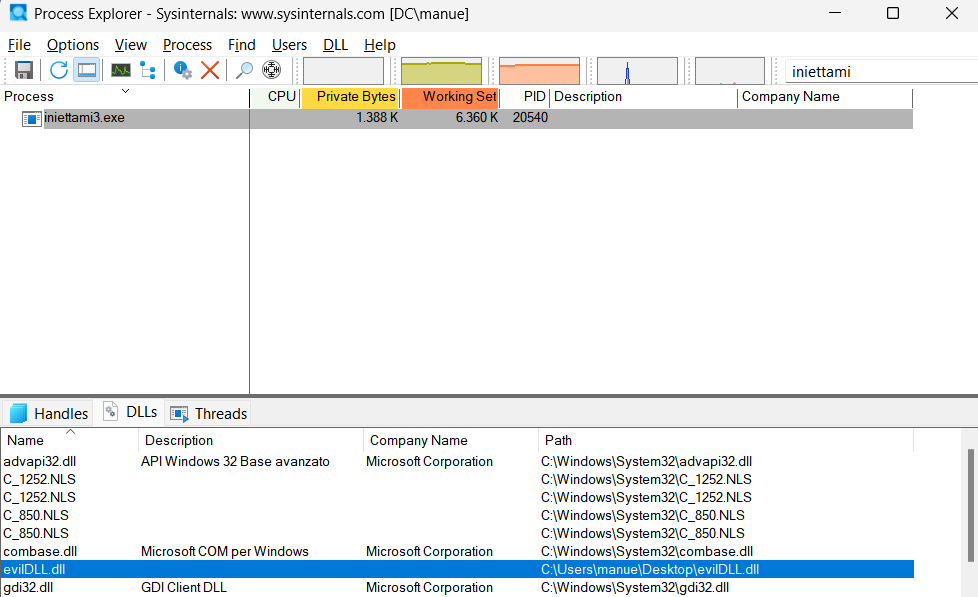
\includegraphics[width=\textwidth,height=7cm]{res/fig/hook-dll.png}
    \caption{DLL all'interno del processo monitorato.}
    \label{fig:hook1}
\end{figure}

\begin{figure}[hbtp]
    \centering
    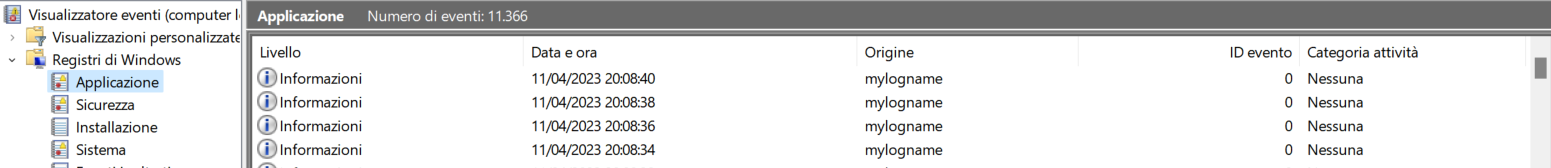
\includegraphics[width=\textwidth]{res/fig/hook-evento.png}
    \caption{generazione di evento in Windows Event Log System.}
    \label{fig:hook2}
\end{figure}
\begin{figure}[hbtp]
    \centering
    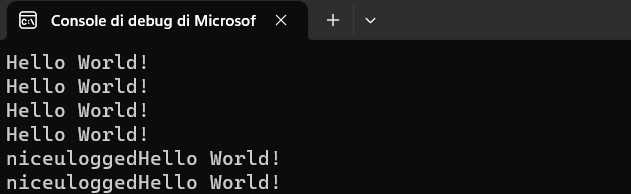
\includegraphics[width=\textwidth,height=5cm]{res/fig/hook-console.png}
    \caption{console del processo prima e dopo l'hook.}
    \label{fig:hook3}
\end{figure}

Estendendo l'idea di fondo del prototipo si potrebbe iniettare una DLL all'interno di ogni nuovo processo alla ricerca di pattern nelle API call, ed eventualmente generare dei log all'interno del Windows Event Log System  così da poterli analizzare attraverso Wazuh.

%inserire esempio behavior based
\medskip
Un'applicazione del concetto di monitoraggio delle system call molto interessante è stata effettuata da Creech e Gideon \cite{creech2014developing}, che hanno sfruttato tale concetto per creare un HIDS che rilevasse anomalie nelle chiamate effettuate.